%%%%%%%%%%%%%%%%%%%%%%%%%%%%%%%%%%%%%%%%%%%%
\section{air4children}


\begin{frame}
      \frametitle{Table of Contents}
      \tableofcontents[currentsection]
\end{frame}


%%%%%%%%%%%%%%%%%%%%%%%%%%%%%%%%%%%%%%%%%%%%%
\subsection{Open source software and hardware in AI and Robotics}

%%%%%%%%%%%%%%%%%%%%%%%%%%%%%%%%%%%%%%%%%%%%%%%%%%%%%%%%
{
%\paper{Savage N. 2021 in Nature}
\begin{frame}{Open source software and hardware in AI and Robotics}

      \begin{figure}
        \centering
        \includegraphics[width=1.0\textwidth]{timeline-osh/outputs/drawing-v00.png}
        %\caption{}
      \end{figure}
\end{frame}
}

%%%%%%%%%%%%%%%%%%%%%%%%%%%%%%%%%%%%%%%%%%%%%%%%%%%%%%%%
{
%\paper{Lastname N. YEAR in journal of...}
\begin{frame}{
air4children, Artificial Intelligence and Robotics for Children
}
 
  \begin{columns}
  \begin{column}{.7\linewidth}

  \begin{itemize}
    \item create a more inclusive, affordable and fair participation of children in AI and Robotics,
    \item create child-centred AI and Robotics curriculums based on Montessori Education, and
    \item build Open source robots to be affordable and fun. 
  \end{itemize}

    \end{column}


  \begin{column}{.4\linewidth}

      \begin{figure}
        \centering
        \includegraphics[width=0.95\textwidth]{logo/outputs/drawing-v00.png}
      \end{figure}

    \end{column}
  \end{columns}

\end{frame}
}




%%%%%%%%%%%%%%%%%%%%%%%%%%%%%%%%%%%%%%%%%%%%%
\subsection{Prototyping and piloting Open Source Robots}

%%%%%%%%%%%%%%%%%%%%%%%%%%%%%%%%%%%%%%%%%%%%%%%%%%%%%%%%
{
\paper{
Xochicale M. June 2014, Proposal of Libre Robotics. 
\faFilePdfO Libre Robotics: \url{https://github.com/air4children/documents/blob/main/latex-librerobotics/LibrERobotics.pdf};
\faYoutube Voice Controlled Low-Cost Robot: \url{https://www.youtube.com/watch?v=f2mCCzVIxe0}
\faYoutube Robot learning: \url{https://www.youtube.com/watch?v=BKWucKcgsP0};
\faYoutube little robot: \url{https://www.youtube.com/watch?v=DexhVz_B8U0}
}
\begin{frame}{Prototyping Open Source Robots (2013 -- 2017)}
      \begin{figure}
        \centering
        \includegraphics[width=1.0\textwidth]{air4children-a/outputs/drawing-v00.png}
        %\caption{}
      \end{figure}
\end{frame}
}

%%%%%%%%%%%%%%%%%%%%%%%%%%%%%%%%%%%%%%%%%%%%%%%%%%%%%%%%
{
\paper{
  Xochicale M. 2015 in Mecate; 
  \faYoutube ROBIT @MECATE 2015 \url{https://www.youtube.com/watch?v=VjVGnwD422g};
  Parra C. et al. 2016, \url{https://www.ottodiy.com/}    
}
\begin{frame}{Piloting robot prototypes (2015 -- 2019)}
      \begin{figure}
        \centering
        \includegraphics[width=1.0\textwidth]{air4children-b/outputs/drawing-v00.png}
        %\caption{}
      \end{figure}
\end{frame}
}

%%%%%%%%%%%%%%%%%%%%%%%%%%%%%%%%%%%%%%%%%%%%%
\subsection{Montessori Education}

%%%%%%%%%%%%%%%%%%%%%%%%%%%%%%%%%%%%%%%%%%%%%%%%%%%%%%%%
{
\paper{
  Elkin, M., Sullivan, A. and Bers, M.U. (2014). Implementing a Robotics Curriculum in an Early Childhood Montessori Classroom. Journal of Information Technology Education: Innovations in Practice, 13(1), 153-169. Informing Science Institute. \url{https://www.learntechlib.org/p/174845}.
  }
\begin{frame}{Montessori Education} 
\vspace{3mm}
%\it{
"The hand is the instrument of the mind."
%} 
%\\
Dr. Maria Montessori (1970-1952).

\vspace{2mm}
    \begin{figure}
        \centering
        \includegraphics[width=1.0\textwidth]{montessori/outputs/drawing-v00.png}
        %\caption{}
      \end{figure}

Children are participating in creative explorations to develop fine motor skills and to engage in collaborative and teamwork activities. 

\end{frame}
}



%%%%%%%%%%%%%%%%%%%%%%%%%%%%%%%%%%%%%%%%%%%%%%%%%%%%%%%%
{
\paper{
Mohammad Tarik, M., M. Zena Tarik, M. Zahraa Tarek, and M. Farah Tareq. "A Hybrid Spiral Project Based Learning Model for Microprocessor Course Teaching." DOI: \url{http://doi.org/10.24017/kjar}; 
Harden R.M. (1999) What is a spiral curriculum?, Medical Teacher, 21:2, 141-143, DOI: \url{https://doi.org/10.1080/01421599979752}
}    
\begin{frame}{Spiral Learning Method}

  \begin{figure}
        \centering
        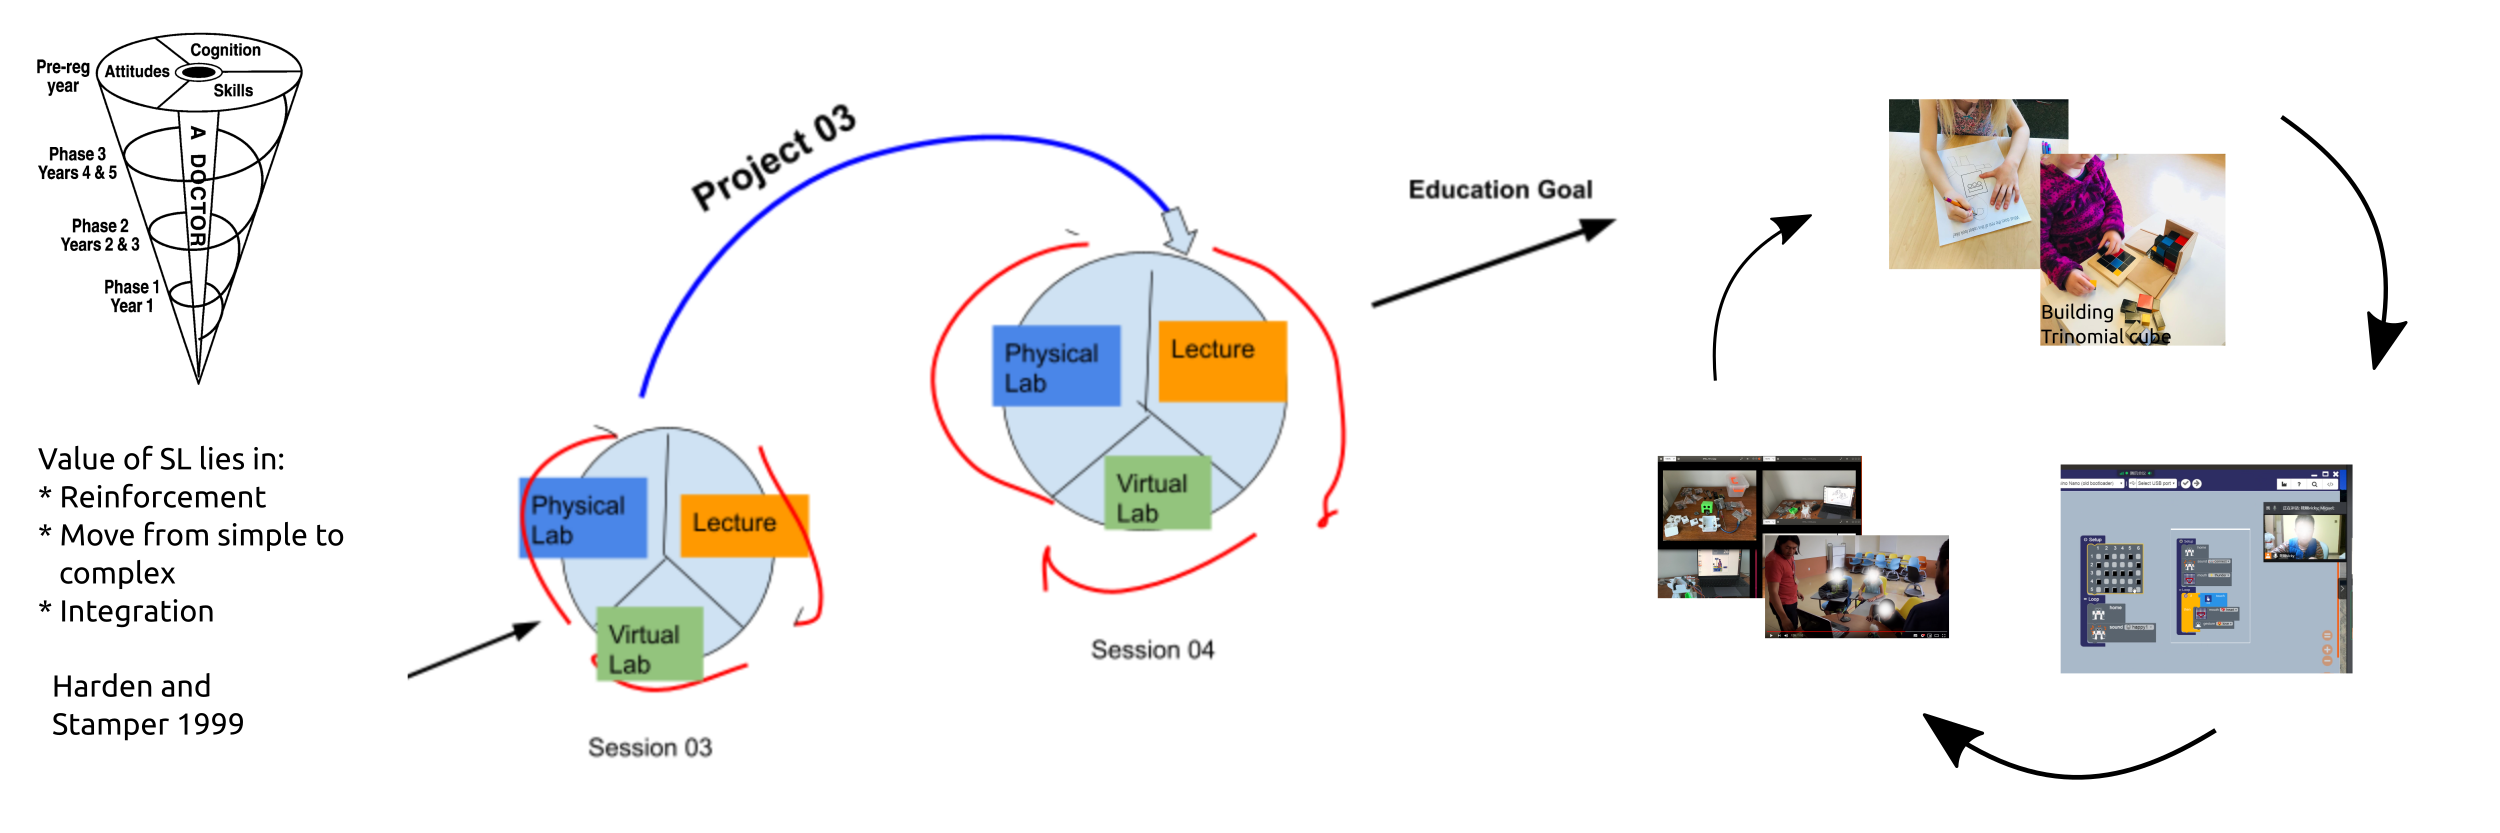
\includegraphics[width=1.0\textwidth]{teaching-materials/outputs/drawing-v02.png}
        %\caption{}
      \end{figure}
\end{frame}
}
